%% -*- coding:utf-8 -*-
\chapter{Neural network basics}

\section{Logistic regression}
Lets consider a simple example of logistic regression that can be used for
classification task. I.e. it will provide \textbf{yes} or \textbf{no} answer on
a question about input data.

Suppose our input data are represented as the following vector
\[
\vec{x} =
\begin{bmatrix}
  x_{1} \\
  x_{2} \\
  \vdots \\
  x_{n}
\end{bmatrix}
\]
The result is a scalar $y \in \{1,0\}$

In the model of supervised learning we have a set of $m$ samples that are used
for learning process:
\[
\begin{array}{c}
  \vec{x}^{(1)} \rightarrow y^{(1)}, \\
  \vec{x}^{(2)} \rightarrow y^{(2)}, \\
  \vdots \\
  \vec{x}^{(m)} \rightarrow y^{(m)}
\end{array}
\]
We want to construct a function $\mathcal{Y}$ such that
\[
\mathcal{Y}\left(\vec{x}^{(i)}\right) = y^{(i)}
\]
for all $i \in \{1, \dots, m\}$. Taking into consideration that the result is a
binary function, we can interpret $\mathcal{Y}$ as a probability that the
outcome will be 1, i.e.
\begin{equation}
  \mathcal{Y}\left(\vec{x}\right) = p\left(\left. y = 1\right|\vec{x}\right)
  \label{eq:ch1:sec1:y_as_probability}
\end{equation}
from \cref{eq:ch1:sec1:y_as_probability} we can derive
\begin{align}
  p\left(\left. y = 1\right|\vec{x}\right) = \mathcal{Y}\left(\vec{x}\right),
  \nonumber \\
  p\left(\left. y = 0\right|\vec{x}\right) = 1 - p\left(\left. y =
  1\right|\vec{x}\right) =
  \nonumber \\
  = 1 - \mathcal{Y}\left(\vec{x}\right)
  \nonumber
\end{align}
Thus we can conclude that
\begin{align}
  p\left(\left. y\right|\vec{x}\right) =
  p\left(\left. y = 1\right|\vec{x}\right)^y \cdot
  p\left(\left. y = 0\right|\vec{x}\right)^{1-y} =
  \nonumber \\
  = \mathcal{Y}\left(\vec{x}\right)^y \cdot
  \left(1 - \mathcal{Y}\left(\vec{x}\right)\right)^{1 - y}
\label{eq:ch1:sec1:probability}
\end{align}
For any test input $\vec{x}^{(i)} \rightarrow y^{(i)}$ we want to maximize the
probability \cref{eq:ch1:sec1:probability}. Taking into consideration that
$p \ge 0$ and $\log$ is a monotonic function \cite{wiki:monotonic_func} then we
can conclude that we want 
to maximize $\log p$ or
\begin{equation}
\log p = y \cdot \log\left(\mathcal{Y}\left(\vec{x}\right)\right) +
(1-y) \log\left(1 - \mathcal{Y}\left(\vec{x}\right)\right)
\label{eq:ch1:sec1:logp}
\end{equation}
Instead of maximizing $\log p$ \cref{eq:ch1:sec1:logp} we can minimize $- \log
p$. Thus we will want to 
minimize the following cost function
\begin{equation}
  \mathcal{L} = - y \cdot \log \left(\mathcal{Y}\left(\vec{x}\right)\right) -
(1-y) \log\left(1 - \mathcal{Y}\left(\vec{x}\right)\right)
  \label{eq:ch1:sec1:cost_func}
\end{equation}
That is similar to Shannon entropy \cite{wiki:entropy_information}.

We want to minimize \cref{eq:ch1:sec1:cost_func} for each test input i.e.
\begin{equation}
  \mathcal{L}^{(i)} = - y^{(i)} \cdot \log\left(\mathcal{Y}\left(\vec{x}^{(i)}\right)\right) -
(1-y^{(i)}) \log \left(1 - \mathcal{Y}\left(\vec{x}^{(i)}\right)\right)
  \label{eq:ch1:sec1:cost_func_i}
\end{equation}
The \cref{eq:ch1:sec1:cost_func_i} can be combined into total cost function as
follows
\begin{equation}
  \mathcal{L} = - \frac{1}{m} \sum_{i = 1}^{m} \left[ y^{(i)} \cdot \log \left(\mathcal{Y}\left(\vec{x}^{(i)}\right)\right) +
(1-y^{(i)}) \log \left(1 - \mathcal{Y}\left(\vec{x}^{(i)}\right)\right)\right]
  \label{eq:ch1:sec1:cost_func_total}
\end{equation}

we have not spoke about $\mathcal{Y}$ so far. Lets assume a linear dependency
for it. it will consists of 2 functions: $\mathcal{Z}$ and $\sigma$. The first
one is the $\mathcal{Z}$ that can be defined as follows
\begin{equation}
  \mathcal{Z} = \vec{\omega}^T \vec{x} + b,
  \label{eq:ch1:sec1:z}
\end{equation}
where
\[
\vec{\omega} =
\begin{bmatrix}
  \omega_{1} \\
  \omega_{2} \\
  \vdots \\
  \omega_{n}
\end{bmatrix}
\]
i.e. the vector of the same dimension as $\vec{x}$.
The equation \cref{eq:ch1:sec1:z} can be rewritten as follows
\[
\mathcal{Z} = \sum_{j = 1} \omega_j x_j +b
\]
and can be considered as a linear form on ${x_j}$. The \cref{eq:ch1:sec1:z}
cannot be interpret as a probability and we need a special function apply on it
that is monotonic \cite{wiki:monotonic_func} and has its value between 0 and
1. The sigmoid function is our choice:
\[
\sigma\left(z\right) = \frac{1}{1+e^{-z}}
\]
Combining all together we can write
\begin{equation}
  \mathcal{Y}\left(\vec{\omega}, b, \vec{x}\right) =
  \sigma\left(\vec{\omega}^T \vec{x} + b\right)
  \label{eq1:ch1:sec1:y_final}
\end{equation}
The form \cref{eq1:ch1:sec1:y_final} is useful for computational purposes as
soon as modern computer uses SIMD (single instruction multiple data) instraction
set that allows to implement vector operations extremely efficient.

We have parameters $\omega_1, \dots, \omega_n, b$ as unknown in
\cref{eq1:ch1:sec1:y_final}. We want to find them by finding a minimum for cost
function \cref{eq:ch1:sec1:cost_func_total}.

Contrary to \cref{eq1:ch1:sec1:y_final}, our cost function is a function of
unknown parameters only:
\begin{align}
  \mathcal{L}\left(\omega_1, \dots, \omega_n, b\right) = - \frac{1}{m} \sum_{i =
    1}^{m} \left[ y^{(i)} \cdot \log \left(\mathcal{Y}\left(\omega_1, \dots, \omega_n, b,
    \vec{x}^{(i)}\right)\right) + \right.
    \nonumber \\
    \left. + 
(1-y^{(i)}) \log \left(1 - \mathcal{Y}\left(\omega_1, \dots, \omega_n, b, \vec{x}^{(i)}\right)\right)\right]
  \label{eq:ch1:sec1:cost_func_total_params}
\end{align}

\begin{figure}
  \centering
  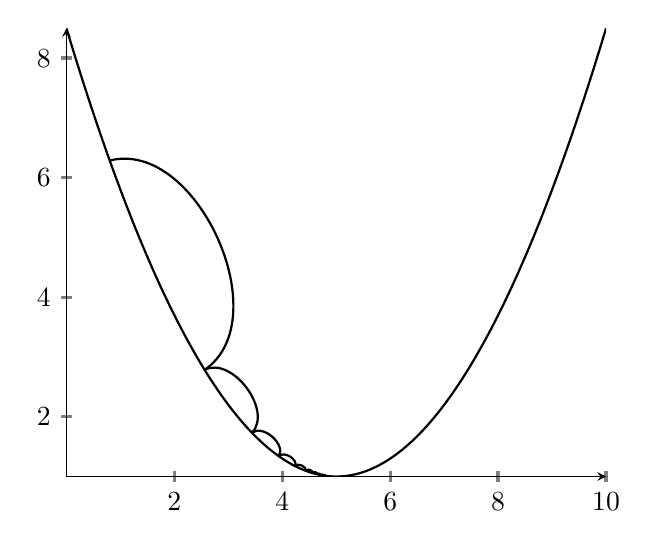
\begin{tikzpicture}
    \begin{axis}[
        axis lines=middle,
        tick style={very thick},
      ]
      %
      %line of best fit
      \addplot[thick,samples=151,domain=0:10] {0.3*(x-5)^(2) + 1}
      foreach \x in {1,...,12} {coordinate[pos={0.5-1.5/pow(1+\x,2)}] (p\x)
        \ifnum\x>1
        (p\the\numexpr\x-1) edge[bend left=80] (p\x)
        \fi};
    \end{axis}
  \end{tikzpicture}
  \caption{Gradient descent}
  \label{fig:ch1:sec1:gradient_desc}
\end{figure}

For finding a minimum of $\mathcal{L}\left(\omega_1, \dots, \omega_n, b\right)$
we can start with any point \cref{fig:ch1:sec1:gradient_desc}, for instance $\omega_j = 0, \forall j$ and $b = 0$
as well. Then we should move in the direction opposite to gradient:
\begin{align}
  \omega_j^{(k)} = \omega_j^{(k-1)} - \alpha \frac{\partial
    \mathcal{L}}{\partial \omega_j}\left(\omega_1^{(k-1)}, \cdots,
  \omega_n^{(k-1)}, b^{(k-1)}\right),
  \nonumber \\
  b^{(k)} = b^{(k-1)}  - \alpha \frac{\partial
    \mathcal{L}}{\partial b}\left(\omega_1^{(k-1)}, \cdots,
  \omega_n^{(k-1)}, b^{(k-1)}\right)
  \nonumber
\end{align}
where $\alpha$ is a parameter that relegates how fast we move to the minimum,
$k$ is the iteration counter.

Thus to find the final formula we have to calculate the derivatives. Lets
rewrite our cost function \cref{eq:ch1:sec1:cost_func_total_params} for the
easiest calculations
\begin{align}
  \mathcal{L}\left(\omega_1, \dots, \omega_n, b\right) =
  \nonumber \\
  = - \frac{1}{m} \sum_{i =
    1}^{m} \left[ y^{(i)} \cdot \log \left(\mathcal{Y}\left(\omega_1, \dots, \omega_n, b,
    \vec{x}^{(i)}\right)\right) + \right .
    \nonumber \\
    + \left .
(1-y^{(i)}) \log \left(1 - \mathcal{Y}\left(\omega_1, \dots, \omega_n, b,
    \vec{x}^{(i)}\right)\right)\right] =
  \nonumber \\
  =
  - \frac{1}{m} \sum_{i =1}^{m} \left[
    y^{(i)} \log \left[\sigma\left(
      \sum_{j=1}^n \omega_j x_j^{(i)} + b\right)\right] +
    \right.
    \nonumber \\
    \left.
    +
(1-y^{(i)}) \log \left[1 - \sigma\left(
    \sum_{j=1}^n \omega_j x_j^{(i)} + b\right)\right]\right]
  \nonumber
\end{align}
For instance
\begin{equation}
 \frac{\partial
   \mathcal{L}}{\partial \omega_j} =
 - \frac{1}{m} \sum_{i =
    1}^{m} \left[ y^{(i)} \frac{1}{\sigma}\frac{d \sigma}{d z}\frac{\partial
     z}{\partial \omega_j} - 
(1-y^{(i)}) \frac{1}{1 - \sigma}\frac{d \sigma}{d z}\frac{\partial
     z}{\partial \omega_j}\right]
 \nonumber
\end{equation}
where we used
\[
\left(\log\left(f\right)\right)' = \frac{f'}{f} 
\]
and used $z$ as
\[
z = \sum_{j=1}^n \omega_j x_j^{(i)} +b 
\]
i.e.
\begin{equation}
  \frac{\partial z}{\partial \omega_j} = x_j^{(i)}
  \nonumber
\end{equation}
from the other size
\begin{align}
  \frac{d \sigma}{d z} = - \frac{1}{\left(1 + e^{-z}\right)^2} \cdot \left( -
  e^{-z}\right) =
  \nonumber \\
  = \frac{1}{\left(1 + e^{-z}\right)^2} \left(1 - \frac{1}{1 +
    e^{-z}}\right)\left(1 + e^{-z}\right) =
  \nonumber \\
  = \frac{1}{1 + e^{-z}} \left(1 - \frac{1}{1 +
    e^{-z}}\right) = \sigma(z) \left(1 - \sigma(z)\right).
  \nonumber 
\end{align}
Thus
\begin{align}
 \frac{\partial
   \mathcal{L}}{\partial \omega_j} =
 - \frac{1}{m} \sum_{i =
    1}^{m} \left[ y^{(i)} x_j^{(i)} (1-\sigma(z)) - 
(1-y^{(i)}) x_j^{(i)} \sigma(z)\right] =
 \nonumber \\
 =
 - \frac{1}{m} \sum_{i =1}^{m}
 \left[ y^{(i)} x_j^{(i)} -\sigma(z) y^{(i)} x_j^{(i)} -
   x_j^{(i)} \sigma(z) + y^{(i)} x_j^{(i)} \sigma(z)\right] =
 \nonumber \\
 =
 - \frac{1}{m} \sum_{i = 1}^{m}
 \left[ y^{(i)} x_j^{(i)} - x_j^{(i)} \sigma(z) \right] =
  - \frac{1}{m} \sum_{i = 1}^{m} x_j^{(i)} \left[ y^{(i)} - \sigma(z) \right] =
  \nonumber \\
  = \frac{1}{m} \sum_{i = 1}^{m} x_j^{(i)} \left[ \sigma(z) - y^{(i)} \right]
  \nonumber
\end{align}
where
\[
\sigma(z) = \sigma\left(\vec{\omega}^T\vec{x}^{(i)} + b\right).
\]
For derivative by $b$ we have
\[
\frac{\partial \sigma}{\partial b} = 1,
\]
thus
\begin{equation}
 \frac{\partial
   \mathcal{L}}{\partial b} =
  \frac{1}{m} \sum_{i = 1}^{m} \left[ \sigma(z) - y^{(i)} \right]
 \nonumber
\end{equation}

%% TBD
